\documentclass[conference]{IEEEtran}
\IEEEoverridecommandlockouts
% The preceding line is only needed to identify funding in the first footnote. If that is unneeded, please comment it out.
\usepackage{cite}
\usepackage{amsmath,amssymb,amsfonts}
\usepackage{algorithmic}
\usepackage{graphicx}
\usepackage{textcomp}
\usepackage{xcolor}
\usepackage{titlesec}
\def\BibTeX{{\rm B\kern-.05em{\sc i\kern-.025em b}\kern-.08em
    T\kern-.1667em\lower.7ex\hbox{E}\kern-.125emX}}
\begin{document}

\title{Reinforcement Learning in Strategy-Based and Atari Games: A Review of Google DeepMind's Innovations\\}

\IEEEoverridecommandlockouts

\author{
    \IEEEauthorblockN{
        \parbox{.45\textwidth}{\centering
            Abdelrhman Shaheen\\
            \textit{Computer Science Engineering Undergraduate Student} \\
            \textit{Egypt Japan University of Science and Technology} \\
            Alexandria, Egypt \\
            abdelrhman.shaheen@ejust.edu.eg
        }
        \hfill
        \parbox{.45\textwidth}{\centering
            Anas Badr\\
            \textit{Computer Science Engineering Undergraduate Student} \\
            \textit{Egypt Japan University of Science and Technology} \\
            Alexandria, Egypt \\
            anas.badr@ejust.edu.eg
        }
    }
    \\[0.5cm]
    \IEEEauthorblockN{
        \parbox{.45\textwidth}{\centering
            Ali Abohendy\\
            \textit{Computer Science Engineering Undergraduate Student} \\
            \textit{Egypt Japan University of Science and Technology} \\
            Alexandria, Egypt \\
            ali.abohendy@ejust.edu.eg
        }
        \hfill
        \parbox{.45\textwidth}{\centering
            Hatem Alsaadawy\\
            \textit{Computer Science Engineering Undergraduate Student} \\
            \textit{Egypt Japan University of Science and Technology} \\
            Alexandria, Egypt \\
            hatem.alsaadawy@ejust.edu.eg
        }
    }
    \\[0.5cm]
    \IEEEauthorblockN{
        \parbox{.45\textwidth}{\centering
            Nadine Alsayad\\
            \textit{Computer Science Engineering Undergraduate Student} \\
            \textit{Egypt Japan University of Science and Technology} \\
            Alexandria, Egypt \\
            nadine.alsayad@ejust.edu.eg
        }
        \hfill
        \parbox{.45\textwidth}
    }
}


\maketitle

\begin{abstract}

    Abstract

\end{abstract}

\begin{IEEEkeywords}
    Deep Reinforcement Learning, Google DeepMind, AlphaGo, AlphaGo Zero, MuZero, Atari Games, Go, Chess, Shogi,
\end{IEEEkeywords}

\section{Introduction}
%Introcution section%
Artificial Intelligence (AI) has revolutionized the gaming industry, both as a
tool for creating intelligent in-game opponents and as a testing environment
for advancing AI research. Games serve as an ideal environment for training and
evaluating AI systems because they provide well-defined rules, measurable
objectives, and diverse challenges. From simple puzzles to complex strategy
games, AI research in gaming has pushed the boundaries of machine learning and
reinforcement learning. Also The benfits from such employment helped game
developers to realize the power of AI methods to analyze large volumes of
player data and optimize game designs. \cite{I1} \\ Atari games, in particular,
with their retro visuals and straightforward mechanics, offer a challenging yet
accessible benchmark for testing AI algorithms. The simplicity of Atari games
hides complexity that they require strategies that involve planning,
adaptability, and fast decision-making, making them also a good testing
environment for evaluating AI's ability to learn and generalize. The
development of AI in games has been a long journey, starting with rule-based
systems and evolving into more sophisticated machine learning models. However,
the machine learning models had a few challenges, from these challenges is that
the games employing AI involves decision making in the game evironment. Machine
learning models are unable to interact with the decisions that the user make
because it depends on learning from datasets and have no interaction with the
environment. To overcome such problem, game developers started to employ
reinforcement learning (RL) in developing games. Years later, deep learning
(DL) was developed and shows remarkable results in video games\cite{I2}. The
combination between both reinforcement learning and deep learning resulted in
Deep Reinforcement Learning (DRL). The first employment of DRL was by game
developers in atari game\cite{I3}. One of the famous companies that employed
DRL in developing AI models is Google DeepMind. This company is known for
developing AI models, including games. Google DeepMind passed through a long
journey in developing AI models for games. Prior to the first DRL game model
they develop, which is AlphaGo, Google DeepMind gave a lot of contributions in
developing DRL, by which these contributions were first employed in Atari
games.\\ For the employment of DRL in games to be efficient, solving tasks in
games need to be sequential, so Google DeepMind combined RL-like techniques
with neural networks to create models capable of learning algorithms and
solving tasks that require memory and reasoning, which is the Neural Turing
Machines (NTMs)\cite{I4}. They then introduced the Deep Q-network (DQN)
algorithm, which is combine deep learning with Q-learning and RL algorithm.
Q-learning is a model in reinforcement learning which use the Q-network, which
is is a type of neural network to approximate the Q-function, which predicts
the value of taking a particular action in a given state\cite{I5}. The DQN
algorithm was the first algorithm that was able to learn directly from
high-dimensional sensory input, the data that have a large number of features
or dimensions\cite{I6}.\\ To enhance the speed of learning in reinforcement
learning agents, Google DeepMind introduced the concept of experience replay,
which is a technique that randomly samples previous experiences from the
agent's memory to break the correlation between experiences and stabilize the
learning process\cite{I7}. They then developed asynchronus methods for DRL,
which is the Actor-Critic (A3C) model. This model showed faster and more stable
training and showed a remarkable performance in Atari games\cite{I8}. By the
usage of these algorithms, Google DeepMind was able to develop the first AI
model that was able to beat the world champion in the game of Go, which is
AlphaGo in 2016.\\
The paper is organized as follows: Section II presents the related work that
surveys the development of DRL in games and the contribution that we 
added to the previous surveys. Section III presents the background 
information about the development of DRL in games. Section IV presents the
first AI model that Google DeepMind developed, which is AlphaGo. Section V
presents AlphaGo Zero. Section VI presents MuZero. Section VII presents the
advancements that were made in developing AI models for games. Section VIII 
presents the future directions that AI models for games will take, and their
applications in real life.

\section{Background}

%BACKGROUND SECTION%
\renewcommand\theparagraph{\arabic{subsubsection}.\arabic{paragraph}}
\titleformat{\paragraph}[hang]{\normalfont\normalsize\bfseries}{\theparagraph}{1em}{}
\titlespacing*{\paragraph}{2em}{0.5ex plus 0.2ex minus .2ex}{0em}

Reinforcement Learning (RL) is a key area of machine learning that focuses on
learning through interaction with the environment. In RL, an agent takes
actions (A) in specific states (S) with the goal of maximizing the rewards (R)
received from the environment. The foundations of RL can be traced back to
1911, when Thorndike introduced the Law of Effect, suggesting that actions
leading to favorable outcomes are more likely to be repeated, while those
causing discomfort are less likely to recur \cite{bg1}.\\ RL emulates the human
learning process of trial and error. The agent receives positive rewards for
beneficial actions and negative rewards for detrimental ones, enabling it to
refine its policy function—a strategy that dictates the best action to take in
each state. That's said, for a give agent in state $u$, if it takes action $u$,
then the immediate reward $r$ can be modeled as $r(x, u) = \mathbb{E}[r_t \mid
    x=x_{t-1}, u=u_{t-1}]$.\\ So for a full episode of $T$ steps, the cumulative
reward $R$ can be modeled as $R = \sum_{t=1}^{T} r_t$.\\
\subsection{Markov Decision Process (MDP)}

In reinforcement learning, the environment is often modeled as a \textbf{Markov
    Decision Process (MDP)}, which is defined as a tuple $(S, A, P, R, \gamma)$,
where:
\begin{itemize}
    \item \( S \) is the set of states,
    \item \( A \) is the set of actions,
    \item \( P \) is the transition probability function,
    \item \( R \) is the reward function, and
    \item \( \gamma \) is the discount factor.
\end{itemize}

The MDP framework is grounded in \textbf{sequential decision-making}, where the
agent makes decisions at each time step based on its current state. This
process adheres to the \textbf{Markov property}, which asserts that the future
state and reward depend only on the present state and action, not on the
history of past states and actions.

Formally, the Markov property is represented by:

\begin{equation}
    P(s'\mid s, a) = \mathbb{P}[s_{t+1} = s' \mid s_t = s, a_t = a]
\end{equation}

which denotes the probability of transitioning from state $s$ to state $s'$
when action $a$ is taken.

The reward function \( R \) is similarly defined as:

\begin{equation}
    R(s, a) = \mathbb{E}[r_t \mid s_{t-1} = s, a_{t-1} = a]
\end{equation}

which represents the expected reward received after taking action $a$ in state
$S$.
\subsection{Policy and Value Functions}
In reinforcement learning, an agent's goal is to find the optimal policy that
the agent should follow to maximize cumulative rewards over time. To facilitate
this process, we need to quantify the desirability of a given state, which is
done through the \textbf{value function} $V(s)$. Value function estimates the
expected cumulative reward an agent will receive starting from state \( s \)
and continuing thereafter. In essence, the value function reflects how
beneficial it is to be in a particular state, guiding the agent's
decision-making process. The \textbf{state-value function} is then defined as:

\begin{equation}\label{eq:v_pi}
    \begin{split}
        V_\pi(s) & = \mathbb{E_\pi}[G_t \mid s_t = s]                            \\
                 & = \mathbb{E_\pi}[r_t + \gamma r_{t+1}  + \ldots \mid s_t = s]
    \end{split}
\end{equation}

where \( G_t \) is the cumulative reward from time step $t$ onwards. From here
we can define another value function the \textbf{action-value function} under
policy $\pi$, which is $Q_\pi(s, a)$, that estimates the expected cumulative
reward from the state $s$ and taking action $a$ and then following policy
$\pi$:

\begin{equation}\label{eq:q_pi}
    \begin{split}
        Q_\pi(s, a) & = \mathbb{E_\pi}[G_t \mid s_t = s, a_t = a]                            \\
                    & = \mathbb{E_\pi}[r_t + \gamma r_{t+1}  + \ldots \mid s_t = s, a_t = a]
    \end{split}
\end{equation}

where $\gamma$ is the discount factor, which is a decimal value between 0 and 1
that detemines how much we care about immediate rewards versus future reward
rewards \cite{bg2}.\\

We say that a policy $\pi$ is better than another policy $\pi'$ if the expected
return of every state under $\pi$ is greater than or equal to the expected
return of every state under $\pi'$, i.e., $V_\pi(s) \geq V_{\pi'}(s)$ for all
$s \in S$. Eventually, there will be a policy (or policies) that are better
than or equal to all other policies, this is called the \textbf{optimal policy}
$\pi^*$. All optimal policies will then share the same optimal state-value
function $V^*(s)$ and the same optimal action-value function $Q^*(s, a)$, which
are defined as:

\begin{equation}
    \begin{split}
        V^*(s)    & = \max_\pi V_\pi(s)    \\
        Q^*(s, a) & = \max_\pi Q_\pi(s, a)
    \end{split}
\end{equation}

If we can estimate the optimal state-value (or action-value) function, then the
optimal policy $\pi^*$ can be obtained by selecting the action that maximizes
the state-value (or action-value) function at each state, i.e., $\pi^*(s) =
    \arg\max_a Q^*(s, a)$ and that's the goal of reinforcement learning\cite{bg2}.

\subsection{Reinforcement Learning Algorithms}
There are multiple reinforcement learning algorithms that have been developed
that falls under a lot of categories. But, for the sake of this review, we will
focus on the following algorithms that have been used by the Google DeepMind
team in their reinforcement learning models.\\

\subsubsection{\textbf{Model-Based Algorithms: Dynamic Programming}}

\hspace{1em} Dynamic programming (DP) algorithms can be applied when we have a perfect model
of the environment, represented by the transition probability function \( P(s',
r \mid s, a) \). These algorithms rely on solving the Bellman equations
(recursive form of equations \ref{eq:v_pi} and \ref{eq:q_pi}) iteratively to
compute optimal policies. The process alternates between two key steps:
\textbf{policy evaluation} and \textbf{policy improvement}.

\paragraph{Policy Evaluation}
Policy evaluation involves computing the value function \( V^\pi(s) \) under a
given policy \( \pi \). This is achieved iteratively by updating the value of
each state based on the Bellman equation:
\begin{equation}
    V^\pi(s) = \sum_{a \in A} \pi(a \mid s) \sum_{s', r} P(s', r \mid s, a) \left[ r + \gamma V^\pi(s') \right].
\end{equation}

Starting with an arbitrary initial value \( V^\pi(s) \), the updates are
repeated for all states until the value function converges to a stable
estimate.

\paragraph{Policy Improvement}
Once the value function \( V^\pi(s) \) has been computed, the policy is
improved by choosing the action \( a \) that maximizes the expected return for
each state:
\begin{equation}
    \pi'(s) = \arg\max_a \sum_{s', r} P(s', r \mid s, a) \left[ r + \gamma V^\pi(s') \right].
\end{equation}

This step ensures that the updated policy \( \pi' \) is better than or equal to
the previous policy \( \pi \). The process alternates between policy evaluation
and improvement until the policy converges to the optimal policy \( \pi^* \),
where no further improvement is possible. It can be visualized as:

\[
    \pi_0 \xrightarrow{\text{Eval}} V^{\pi_0} \xrightarrow{\text{Improve}} \pi_1 \xrightarrow{\text{Eval}} V^{\pi_1} \xrightarrow{\text{Improve}} \pi_2 \xrightarrow{\text{Eval}} \ldots \xrightarrow{\text{Improve}} \pi^*.
\]

\paragraph{Value Iteration}
Value iteration simplifies the DP process by combining policy evaluation and
policy improvement into a single step. Instead of evaluating a policy
completely, it directly updates the value function using:
\begin{equation}
    V^*(s) = \max_a \sum_{s', r} P(s', r \mid s, a) \left[ r + \gamma V^*(s') \right].
\end{equation}

This method iteratively updates the value of each state until convergence and
implicitly determines the optimal policy. Then the optimal policy can be
obtained by selecting the action that maximizes the value function at each
state, as
\begin{equation}
    \pi^*(s) = \arg\max_a \sum_{s', r} P(s', r \mid s, a) \left[ r + \gamma V^*(s') \right].
\end{equation}

Dynamic Programming's systematic approach to policy evaluation and improvement
forms the foundation for the techniques that have been cruical in training
systems like AlphaGo Zero and MuZero.

\subsubsection{\textbf{Model-Free Algorithms}}

\paragraph{Monte Carlo Algorithm (MC)}
The Monte Carlo (MC) algorithm is a model-free reinforcement learning method
that estimates the value of states or state-action pairs under a given policy
by averaging the returns of multiple episodes. Unlike DP, MC does not require a
perfect model of the environment and instead learns from sampled experiences.

The key steps in MC include:

\begin{itemize}
    \item \textbf{Policy Evaluation:} Estimate the value of a state or state-action pair \( Q(s, a) \) by averaging the returns observed in multiple episodes.
    \item \textbf{Policy Improvement:} Update the policy \( \pi \) to choose actions that maximize the estimated value \( Q(s, a) \).
\end{itemize}

MC algorithms operate on complete episodes, requiring the agent to explore all
state-action pairs sufficiently to ensure accurate value estimates. The updated
policy is given by:
\begin{equation}
    \pi(s) = \arg\max_a Q(s, a).
\end{equation}

While both MC and DP alternate between policy evaluation and policy
improvement, MC works with sampled data, making it suitable for environments
where the dynamics are unknown or difficult to model.

This algorithm is particularly well-suited for environments that are
\emph{episodic}, where each episode ends in a terminal state after a finite
number of steps. \\ Monte Carlo's reliance on episodic sampling and policy
refinement has directly influenced the development of search-based methods like
Monte Carlo Tree Search (MCTS), which was crucial in AlphaGo for evaluating
potential moves during gameplay. The algorithm's adaptability to model-free
settings has made it a cornerstone of modern reinforcement learning strategies.

\paragraph{Temporal Diffrence (TD)}

Temporal Diffrence is another model free algorithm that's very similar To Monte
Carlo, but instead of waiting for termination of the episode to give the
return, it estimates the return based on the next state. The key idea behind TD
is to update the value function based on the difference between the current
estimate and the estimate of the next state. The TD return is then given by:
\begin{equation}
    G_t = r_{t+1} + \gamma V(s_{t+1})
\end{equation}
that's the target (return value estimation) of state $s$ at time $t$ is the immediate reward $r$ plus the
discounted value of the next state $s_{t+1}$.\\
This here is called the TD(0) algorithm, which is the simplest form of TD
that take only one future step into account. The update rule for TD(0) is:
\begin{equation}
    V(s_t) = V(s_t) + \alpha [r_{t+1} + \gamma V(s_{t+1}) - V(s_t)]
\end{equation}

There are other temporal difference algorithms that works exactly like TD(0),
but with more future steps, like TD($\lambda$). \\

Another important variant of TD is the Q-learning algorithm, which is an
off-policy TD algorithm that estimates the optimal action-value function $Q^*$
by updating the current action value based on the optimal action value of the
next state. The update rule for Q-learning is:

\begin{equation}
    Q(s_t, a_t) = Q(s_t, a_t) + \alpha[r_{t+1} + \gamma \max_a Q(s_{t+1}, a) - Q(s_t, a_t)] .
\end{equation}

and after the algorithm converges, the optimal policy can be obtained by
selecting the action that maximizes the action-value function at each state, as
$\pi^*(s) = \arg\max_a Q^*(s, a)$.

Temporal Difference methods, including Q-learning, play a crucial role in
modern reinforcement learning by enabling model-free value function estimation
and action selection without the need to terminate the episode. In systems like
AlphaGo and MuZero, TD methods are used to update value functions efficiently
and support complex decision-making processes without requiring a model of the
environment.

\subsubsection{\textbf{Deep RL: Deep Q-Network (DQN)}}

Deep Q-Networks (DQN) represent a significant leap forward in the integration
of deep learning with reinforcement learning. DQN extends the traditional
Q-learning algorithm by using a deep neural network to approximate the Q-value
function, which is essential in environments with large state spaces where
traditional tabular methods like Q-learning become infeasible.

In standard Q-learning, the action-value function \(Q(s, a)\) is learned
iteratively based on the Bellman equation, which updates the Q-values according
to the reward received and the value of the next state. However, when dealing
with complex, high-dimensional inputs such as images or unstructured data, a
direct tabular representation of the Q-values is not practical. This is where
DQN comes in: it uses a neural network, typically a convolutional neural
network (CNN), to approximate \(Q(s, a; \theta)\), where \(\theta\) represents
the parameters of the network.

The core ideas behind DQN are similar to those of traditional Q-learning, but
with a few key innovations that address issues such as instability and high
variance during training. The DQN algorithm introduces the following
components:

\begin{itemize}
    \item \textbf{Experience Replay:} To improve the stability of training and to break the correlation between consecutive experiences, DQN stores the agent’s experiences in a replay buffer. Mini-batches of experiences are randomly sampled from this buffer to update the network, which helps in better generalization.
    \item \textbf{Target Network:} DQN uses two networks: the primary Q-network and a target Q-network. The target network is updated less frequently than the primary network and is used to calculate the target value in the Bellman update. This reduces the risk of oscillations and divergence during training.
\end{itemize}

The update rule for DQN is based on the Bellman equation for Q-learning, but
with the neural network approximation:

\begin{equation}
    \begin{split}
         & Q(s_t, a_t; \theta) = Q(s_t, a_t; \theta) +                                                     \\
         & \alpha \left[ r_{t+1} + \gamma \max_{a'} Q(s_{t+1}, a'; \theta^-) - Q(s_t, a_t; \theta) \right]
    \end{split}
\end{equation}

where \( \theta^- \) represents the parameters of the target network. By
training the network to minimize the difference between the predicted Q-values
and the target Q-values, the agent learns an optimal policy over
time.\cite{bg4}

The DQN algorithm revolutionized reinforcement learning, especially in
applications requiring decision-making in high-dimensional spaces. One of the
most notable achievements of DQN was its success in mastering a variety of
Atari 2600 games directly from raw pixel input, achieving human-level
performance across multiple games. This breakthrough demonstrated the power of
combining deep learning with reinforcement learning to solve complex,
high-dimensional problems.

In subsequent improvements, such as Double DQN, Dueling DQN, and Prioritized
Experience Replay, enhancements were made to further stabilize training and
improve performance. However, the foundational concepts of using deep neural
networks to approximate Q-values and leveraging experience replay and target
networks remain core to the DQN framework.


\section{AlphaGo}
\documentclass[conference]{IEEEtran}
\IEEEoverridecommandlockouts
\usepackage{cite}
\usepackage{amsmath,amssymb,amsfonts}
\usepackage{algorithmic}
\usepackage{graphicx}
\usepackage{textcomp}
\usepackage{xcolor}
\def\BibTeX{{\rm B\kern-.05em{\sc i\kern-.025em b}\kern-.08em
    T\kern-.1667em\lower.7ex\hbox{E}\kern-.125emX}}
\begin{document}

\title{AlphaGo: The Intersection of Neural Networks and Monte Carlo Tree Search\\
}

\maketitle


\section{Introduction}
AlphaGo is a groundbreaking reinforcement learning model that utilizes neural networks and tree search to play the game of GO, which is thought to be one of the most challenging classic games for artificial intelligence owing to its enormous search space and the difficulty of evaluating board positions and moves.
\\\\
AlphaGo uses value networks for position evaluation and policy networks for taking actions, that combined with Monte Carlo simulation achieved a 99.8\% winning rate, and beating the European human Go champion in 5 out 5 games.
\section{Key Innovations}

\subsection{Integration of Policy and Value Networks with MCTS}
AlphaGo combines policy and value networks in an MCTS framework to efficiently explore and evaluate the game tree. Each edge \( (s, a) \) in the search tree stores:
\begin{itemize}
    \item Action value \( Q(s, a) \): The average reward for taking action \( a \) from state \( s \).
    \item Visit count \( N(s, a) \): The number of times this action has been explored.
    \item Prior probability \( P(s, a) \): The probability of selecting action \( a \), provided by the policy network.
\end{itemize}

During the selection phase, actions are chosen to maximize:
\[
a_t = \arg\max_a \left( Q(s, a) + u(s, a) \right)
\]
where the exploration bonus \( u(s, a) \) is defined as:
\[
u(s, a) \propto \frac{P(s, a)}{1 + N(s, a)}
\]

When a simulation reaches a leaf node, its value is evaluated in two ways:
1. Value Network Evaluation: A forward pass through the value network predicts \( v_\theta(s) \), the likelihood of winning.
2. Rollout Evaluation: A lightweight policy simulates the game to its conclusion, and the terminal result \( z \) is recorded.

These evaluations are combined using a mixing parameter \( \lambda \):
\[
V(s_L) = \lambda v_\theta(s_L) + (1 - \lambda) z_L
\]

The back propagation step updates the statistics of all nodes along the path from the root to the leaf.


\section{Training Process}

\subsection{Supervised Learning for Policy Networks}
The policy network was initially trained using supervised learning on human expert games. The training data consisted of 30 million board positions sampled from professional games on the KGS Go Server. The goal was to maximize the likelihood of selecting the human move for each position:
\[
\Delta \sigma \propto \nabla_\sigma \log p_\sigma(a | s)
\]
where \( p_\sigma(a | s) \) is the probability of selecting action \( a \) given state \( s \).

This supervised learning approach achieved a move prediction accuracy of 57.0\% on the test set, significantly outperforming prior methods. This stage provided a solid foundation for replicating human expertise.

\subsection{Reinforcement Learning for Policy Networks}
The supervised learning network was further refined through reinforcement learning (RL). The weights of the RL policy network were initialized from the SL network. AlphaGo then engaged in self-play, where the RL policy network played against earlier versions of itself to iteratively improve.

The reward function used for RL was defined as:
\[
r(s) = 
\begin{cases} 
+1 & \text{if win} \\
-1 & \text{if loss} \\
0 & \text{otherwise (non-terminal states).}
\end{cases}
\]
At each time step \( t \), the network updated its weights to maximize the expected reward using the policy gradient method:
\[
\Delta \rho \propto z_t \nabla_\rho \log p_\rho(a_t | s_t)
\]
where \( z_t \) is the final game outcome from the perspective of the current player.

This self-play strategy allowed AlphaGo to discover novel strategies beyond human knowledge. The RL policy network outperformed the SL network with an 80\% win rate and achieved an 85\% win rate against Pachi, a strong open-source Go program, without using MCTS.

\subsection{Value Network Training}
The value network was designed to evaluate board positions by predicting the likelihood of winning from a given state. Unlike the policy network, it outputs a single scalar value \( v_\theta(s) \) between \(-1\) (loss) and \(+1\) (win).

Training the value network on full games led to overfitting due to the strong correlation between successive positions in the same game. To mitigate this, a new dataset of 30 million distinct board positions was generated through self-play, ensuring that positions came from diverse contexts.

The value network was trained by minimizing the mean squared error (MSE) between its predictions \( v_\theta(s) \) and the actual game outcomes \( z \):
\[
L(\theta) = \mathbb{E}_{(s, z) \sim D} \left[ (v_\theta(s) - z)^2 \right]
\]
\section{Challenges and Solutions}
AlphaGo overcame several challenges:
\begin{itemize}
    \item Overfitting: Training the value network on full games led to memorization. This was mitigated by generating a diverse self-play dataset.
    \item Scalability: Combining neural networks with MCTS required significant computational resources, addressed through parallel processing on GPUs and CPUs.
    \item Exploration vs. Exploitation: Balancing these in MCTS was achieved using the exploration bonus \( u(s, a) \) and the policy network priors.
\end{itemize}

\section{Performance Benchmarks}
AlphaGo achieved the following milestones:
\begin{itemize}
    \item 85\% win rate against Pachi without using MCTS.
    \item 99.8\% win rate against other Go programs in a tournament held to evaluate the performance of AlphaGo.
    \item Won 77\%, 86\%, and 99\% of handicap games against Crazy Stone, Zen and Pachi, respectively.
    \item Victory against professional human players such as Fan Hui (5-0) and Lee Sedol (4-1), marking a significant breakthrough in AI.
\end{itemize}
\end{document}



\section{AlphaGo Zero}
\subsubsection{Introduction}
AlphaGo Zero represents a groundbreaking advancement in artificial intelligence
and reinforcement learning. Unlike its predecessor, AlphaGo, which relied on
human gameplay data for training, AlphaGo Zero learns entirely from self-play,
employing deep neural networks and Monte Carlo Tree Search (MCTS). \cite{agz1}
\\\\ By starting with only the rules of the game and leveraging reinforcement
learning, AlphaGo Zero achieved superhuman performance in Go, defeating the
previous version of AlphaGo in a 100-0 match.
\subsubsection{Key Innovations}

AlphaGo Zero introduced several groundbreaking advancements over its
predecessor, AlphaGo, streamlining and enhancing its architecture and training
process:

\begin{enumerate}
    \item Unified Neural Network \( f_\theta \): AlphaGo Zero replaced AlphaGo's
          dual-network setup—separate networks for policy and value—with a single neural
          network \( f_\theta \). This network outputs both the policy vector \( p \) and
          the value scalar \( v \) for a given game state, reprsented as

          \begin{equation}
              f_\theta(s) = (p, v)
          \end{equation}

          This unified architecture simplifies the model and improves training
          efficiency.

    \item Self-Play Training: Unlike AlphaGo, which relied on human games as training
          data, AlphaGo Zero was trained entirely through self-play. Starting from random
          moves, it learned by iteratively playing against itself, generating data and
          refining \( f_\theta \) without any prior knowledge of human strategies. This
          removed biases inherent in human gameplay and allowed AlphaGo Zero to discover
          novel and highly effective strategies.

    \item Removal of Rollouts: AlphaGo Zero eliminated the need for rollouts, which were
          computationally expensive simulations to the end of the game used by AlphaGo's
          MCTS. Instead, \( f_\theta \) directly predicts the value \( v \) of a state,
          providing a more efficient and accurate estimation.

    \item Superior Performance: By integrating these advancements, AlphaGo Zero defeated
          AlphaGo 100-0 in direct matches, demonstrating the superiority of its self-play
          training, unified architecture, and reliance on raw rules over pre-trained
          human data.
\end{enumerate}

\subsubsection{Training Process}

\subsubsubsection{Monte Carlo Tree Search (MCTS) as policy evaluation operator}
Intially the neural network \( f_\theta \) is not very accurate in predicting
the best move, as it is intiallised with random weights at first. To overcome
this, AlphaGo Zero uses MCTS to explore the game tree and improve the policy.
\\\\ At a given state S, MCTS expands simualtions of the best moved that are
most likely to generate a win based on the initial policy $P(s,a)$ and the
value $V$. MCTS iteratively selects moves that maximize the upper confidence
bound (UCB) of the action value. UCB is designed to balanced exploration and
exploitation. and it is defined as

\begin{equation}
    UCB = Q(s, a) + U(s, a)
\end{equation}

where \[U(s, a) \propto \frac{p(s, a)}{1 + N(s, a)}\] MCTS at the end of the search returns the policy vector \( \pi \) which is used
to update the neural network \( f_\theta \) by minimizing the cross-entropy
loss between the predicted policy by $f_\theta$ and the MCTS policy.

\subsubsubsection{Policy Iteration and self play}
The agent uses the MCTS to select the best move at each state and the game is
played till the end in a process called self play. The agent then uses the
outcome of the game, $z$ game winner and $\pi$ to update the neural network.
This process is repeated for a large number of iterations.

\subsubsubsection{Network Training Process}

The neural network is updated after each self-play game by using the data
collected during the game. This process involves several key steps:
\begin{enumerate}
    \item Intilisation of the network: The neural network starts with random weights
          $\theta_0$, as there is no prior knowledge about the game.
    \item Generating Self-play Games: For each iteration $i \geq 1$ self-play games are
          generated. During the game, the neural network uses its current parameters
          $\theta_{i - 1}$ to run MCTS and generate search probabilities $\pi_t$ for each
          move at time step $t$.
    \item Game Termination and scoring: A game ends when either both players pass, a
          resignation threshold is met, or the game exceeds a maximum length. The winner
          of the game is determined, and the final result $z_t$ is recorded, providing
          feedback to the model.
    \item Data Colletion: for each time step $t$, the training data $(s_t, \pi_t, z_t)$
          is stored, where $s_t$ is the game state, $\pi_t$ is the search probabilities,
          and $z_t$ is the game outcome.
    \item Network training process: after collecing data from self-play, The neural
          network $f_\theta$ is adjusted to minimize the error between the predicted
          value v and the self-play winner z, and to maximize the similarity between the
          search probabilities $P$ and the MCTS probabilities. This is done by using a
          loss function that combines the mean-squared error and the cross entropy losses
          repsectibly. The loss function is defined as

          \begin{equation}
              L = (z - v)^2 - \pi^T \log p + c||\theta||^2
          \end{equation}

          where $c$ is the L2 regularization term.

\end{enumerate}

\subsubsection{Challenges and Solutions}
Alpha Go Zero overcame several challanges:
\begin{enumerate}
    \item Human knowledge Dependency: AlphaGo Zero eliminated the need for human gameplay
          data, relying solely on self-play to learn the game of Go. This allowed it to
          discover novel strategies that surpassed human expertise.
    \item Compelxity of the dual network approach in alpha go: AlphaGo utilized separate
          neural networks for policy prediction $p$ and value estimation $V$, increasing
          the computational complexity. AlphaGo Zero unified these into a \textbf{single
              network} that outputs both $p$ and $V$, simplifying the architecture and
          improving training efficiency.
    \item The need of handcrafted features: AlphaGo relied on handcrafted features, such
          as board symmetry and pre-defined game heuristics, for feature extraction.
          AlphaGo Zero eliminated the need for feature engineering by using \textbf{raw
              board states} as input, learning representations directly from the data.
\end{enumerate}

\subsubsection{Performance Benchmarks}

Evaluating the performance of DeepMind’s reinforcement learning (RL) agents for strategy games such as Go has primarily been conducted using Elo ratings and direct head-to-head matches against previous versions. \\

Table \ref{tab:elo_ratings} summarizes the reported Elo ratings of the different versions of AlphaGo, illustrating the rapid progression in strength achieved through successive architectural improvements.

\begin{table}[ht]
\caption{Elo ratings of different AlphaGo versions}
\label{tab:elo_ratings}
\centering
\begin{tabular}{|l|l|}
\hline
Model          & Elo rating \\ \hline
AlphaGo Zero   & 5185       \\ \hline
AlphaGo Master & 4858       \\ \hline
AlphaGo Lee    & 3739       \\ \hline
AlphaGo Fan    & 3144       \\ \hline
\end{tabular}
\end{table}

Additionally, AlphaGo Zero defeated the then state-of-the-art AlphaGo Master in a 100-game match with a score of 89–11, demonstrating the effectiveness of self-play reinforcement learning without the need for Monte Carlo rollouts or human expert data.


\section{MuZero}

% Introduction
\subsection*{Introduction}
Through the development of AlphaZero, a general model for board games with superhuman ability has 
been achieved in three games: Go, chess, and Shogi. It could achieve these results without the need for 
human gameplay data or history, instead using self-play in an enclosed environment. However, the 
model still relied on a simulator that could perfectly replicate the behavior, which might not translate 
well to real-world applications, where modeling the system might not be feasible. MuZero 
was developed to address this challenge by developing a model-based RL approach that could learn 
without explicitly modeling the real environment. This allowed for the same general approach used in 
AlphaZero to be used in Atari environments where reconstructing the environment is costly. Essentially, 
MuZero was deployed to all the games with no prior knowledge of them or specific optimization and 
managed to show state-of-the-art results in almost all of them.

% MuZero Algorithm
\subsection*{MuZero Algorithm}
\begin{figure}[h!]
    \centering
    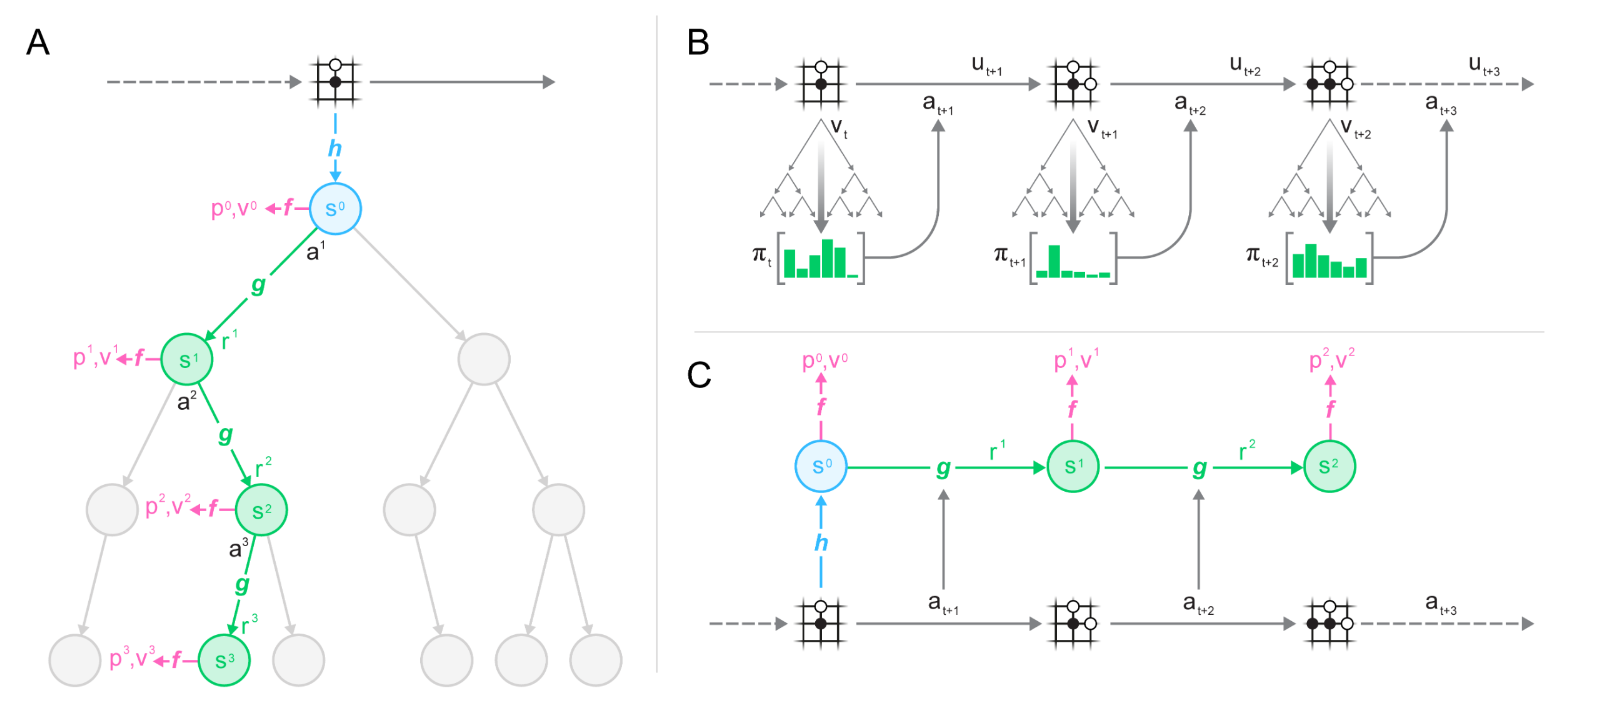
\includegraphics[width=0.35\textwidth]{sections/6MuZero/graph_1.png}
    \caption{(A)The progression of the model through its MDP. (B)MuZero acting as an environment with MCTS as feedback. (C)A diagram of training MuZero's model.}
    \label{fig_1}
\end{figure}
The model takes in an input of observations $o_1, \ldots, o_t$ that are then fed to a representation network $h$, 
which reduces the dimensions of the input and produces a root hidden state $s_0$. Internally, the model 
mirrors an MDP, with each state representing a node with edges connecting it to the future states 
depending on available actions. Unlike traditional RL approaches, this hidden state is not constrained to
contain the information necessary to reproduce the entire future observations. Instead, the hidden states 
are only optimized for predicting information that is related to planning. At every time step, the model 
predicts the policy, the immediate reward, and the value function. The output of the state-action pair is 
then used by the dynamics function to produce future states. Similar to AlphaZero, a Monte Carlo tree 
search is used to find the best action policy given an input space. This is used to train the model by 
comparing the MCTS policy with the predictor function policy. Also, after a few training runs, the model 
ceases to use illegal moves, and the predicted actions map to the real action space. This eliminates the 
need for a simulator, as the model internalizes the environment characteristics it deems necessary for
planning and acting, which generally converges to reality through training. The value function at 
the final step is compared against the game result in board games, i.e., win, loss, or a draw.

\subsection*{Loss function and learning equations}

\begin{align}
    s_0 &= h_\theta(o_1, \ldots, o_t) \\
    r_k, s_k &= g_\theta(s_{k-1}, a_k) \\
    p_k, v_k &= f_\theta(s_k)
\end{align}

\begin{equation}
\setlength{\arraycolsep}{1.5pt} % Reduce spacing inside the matrix
\begin{bmatrix}
    p_k \\ v_k \\ r_k
\end{bmatrix}
=
\mu_\theta(o_1, \ldots, o_t, a_1, \ldots, a_k)
\label{eq:matrix}
\end{equation}

\begin{align}
    \nu_t, \pi_t &= \text{MCTS}(s_0^t, \mu_\theta) \\
    a_t &\sim \pi_t
\end{align}

\begin{align}
    p_k^t, v_k^t, r_k^t &= \mu_\theta(o_1, \ldots, o_t, a_{t+1}, \ldots, a_{t+k}) \\
    z_t &= 
    \begin{cases} 
        u_T, & \text{for games} \\
        u_{t+1} + \gamma u_{t+2} + \ldots \nonumber \\
        \quad + \gamma^{n-1} u_{t+n} + \gamma^n \nu_{t+n}, & \text{for general MDPs}
    \end{cases}
\end{align}

\begin{align}
    l_t(\theta) &=
    \sum_{k=0}^K \big[ l_r(u_{t+k}, r_k^t) + l_v(z_{t+k}, v_k^t) \nonumber \\
    & \quad + l_p(\pi_{t+k}, p_k^t) \big] + c \|\theta\|^2
\end{align}

\begin{align}
    l_r(u, r) &= 
    \begin{cases} 
        0, & \text{for games} \\
        \phi(u)^T \log r, & \text{for general MDPs}
    \end{cases} \\
    l_v(z, q) &= 
    \begin{cases} 
        (z - q)^2, & \text{for games} \\
        \phi(z)^T \log q, & \text{for general MDPs}
    \end{cases} \\
    l_p(\pi, p) &= \pi^T \log p
\end{align}



% MCTS
\subsection*{MCTS}
MuZero uses the same approach developed in AlphaZero to find the optimum action given an internal 
state. MCTS is used where states are the nodes, and the edges store visit count, mean value, policy, and 
reward. The search is done in a three-phase setup: selection, expansion, and backup. The simulation 
starts with a root state, and an action is chosen based on the state-transition reward table. Then, after the end 
of the tree, a new node is created using the output of the dynamics function as a value, and the data from the 
prediction function is stored in the edge connecting it to the previous state. Finally, the simulation 
ends, and the updated trajectory is added to the state-transition reward table. In two-player zero-sum 
games, board games, for example, the value function is bounded between 0 and 1, which is helpful to 
use value estimation and probability using the pUCT rule. However, many other environments have 
unbounded values, so MuZero rescales the value to the maximum value observed by the model up to 
this training step, ensuring no environment-specific data is needed.\cite{mz1}

% Results
\subsection*{Results}
The MuZero model demonstrated significant improvements across various test cases, achieving state-of-the-art performance in several scenarios. Key findings include:

\subsubsection*{Board Games}
\begin{itemize}
    \item When tested on the three board games AlphaZero was trained for (Go, chess, and shogi):
    \begin{itemize}
        \item MuZero matched AlphaZero's performance \textbf{without any prior knowledge} of the games' rules.
        \item It achieved this with \textbf{reduced computational cost} due to fewer residual blocks in the representation function.
    \end{itemize}
\end{itemize}

\subsubsection*{Atari Games}
\begin{itemize}
    \item MuZero was tested on 60 Atari games, competing against both human players and state-of-the-art models (model-based and model-free). Results showed:
    \begin{itemize}
        \item \textbf{Starting from regular positions:} MuZero outperformed competitors in \textbf{46 out of 60 games}.
        \item \textbf{Starting from random positions:} MuZero maintained its lead in \textbf{37 out of 60 games}, though its performance was reduced.
    \end{itemize}
    \item The computational efficiency and generalization of MuZero highlight its effectiveness in complex, unstructured environments.
\end{itemize}

\subsubsection*{Limitations}
\begin{itemize}
    \item Despite its strengths, MuZero struggled in certain games, such as:
    \begin{itemize}
        \item \emph{Montezuma's Revenge} and \emph{Pitfall}, which require long-term planning and strategy.
    \end{itemize}
    \item General challenges:
    \begin{itemize}
        \item Long-term dependencies remain difficult for MuZero, as is the case for RL models in general.
        \item Limited input space and lack of combinatorial inputs in Atari games could introduce scalability issues for broader applications.\cite{mz1}
    \end{itemize}
\end{itemize}




\section{Advancements}
%Advancments%
The evolution of AI in gaming, particularly through the development of AlphaGo,
AlphaGo Zero, and MuZero, highlights remarkable advancements in reinforcement
learning and artificial intelligence. AlphaGo, the pioneering model, combined
supervised learning and reinforcement learning to master the complex game of
Go, setting the stage for AI to exceed human capabilities in well-defined
strategic games. Building on, AlphaGo Zero eliminated the reliance on human
data, introducing a fully self-supervised approach that demonstrated greater
efficiency and performance by learning solely through self-play. MuZero took
this innovation further by generalizing beyond specific games like Go, Chess,
and Shogi, employing model-based reinforcement learning to predict dynamics
without explicitly knowing the rules of the environment. Completing on these
three models, here are some of the advancements that developed from them:
AlphaZero and MiniZero; and one of the most used in generating AI models,
Multi-agent models.
\subsection*{AlphaZero}
While AlphaGo Zero was an impressive feat, designed specifically to master the
ancient game of Go through self-play, AlphaZero developes it by generalizing
its learning framework to include multiple complex games: chess, shogi
(Japanese chess), and Go. The key advancement is in its ability to apply the
same algorithm across different games without requiring game-specific
adjustments. AlphaZero's neural network is trained through self-play,
predicting the move probabilities and game outcomes for various positions. This
prediction is then used to guide the MCTS, which explores potential future
moves and outcomes to determine the best action. Through iterative self-play
and continuous refinement of the neural network, AlphaZero efficiently learns
and improves its strategies across different games\cite{AD3}. Another
significant improvement is in AlphaZero’s generalized algorithm, is that it
does not need to be fine-tuned for each specific game. This was a departure
from AlphaGo Zero’s Go-specific architecture, making AlphaZero a more versatile
AI system.\\ AlphaZero's architecture integrates a single neural network that
evaluates both the best moves and the likelihood of winning from any given
position, streamlining the learning process by eliminating the need for
separate policy and value networks used in earlier systems. This innovation not
only enhances computational efficiency but also enables AlphaZero to adopt
unconventional and creative playing styles that diverge from established human
strategies.
\subsection*{MiniZero}
MiniZero is a a zero-knowledge learning framework that supports four
state-of-the-art algorithms, including AlphaZero, MuZero, Gumbel AlphaZero, and
Gumbel MuZero\cite{AD1}. Gumbel AlphaZero and Gumbel MuZero are variants of the
AlphaZero and MuZero algorithms that incorporate Gumbel noise into their
decision-making process to improve exploration and planning efficiency in
reinforcement learning tasks. Gumbel noise is a type of stochastic noise
sampled from the Gumbel distribution, commonly used in decision-making and
optimization problems.\\ MiniZero is a simplified version of the original
MuZero algorithm, which is designed to be have a more simplified architecture
reducing the complexity of the neural network used to model environment
dynamics, making it easier to implement and experiment with. This
simplification allows MiniZero to perform well in smaller environments with
fewer states and actions, offering faster training times and requiring fewer
computational power compared to MuZero.

\subsection*{Multi-agent models}
Multi-agent models in reinforcement learning (MARL) represent an extension of
traditional single-agent reinforcement learning. In these models, multiple
agents are simultaneously interacting, either competitively or cooperatively,
making decisions that impact both their own outcomes and those of other agents.
The complexity in multi-agent systems arises from the dynamic nature of the
environment, where the actions of each agent can alter the environment and the
states of other agents. Unlike in single-agent environments, where the agent
learns by interacting with a static world, multi-agent systems require agents
to learn not only from their direct experiences but also from the behaviors of
other agents, leading to a more complex learning process. Agents must adapt
their strategies based on what they perceive other agents are doing, and this
leads to problems such as strategic coordination, deception, negotiation, and
competitive dynamics. In competitive scenarios, agents might attempt to outwit
one another, while in cooperative scenarios, they must synchronize their
actions to achieve a common goal\cite{AD2}.\\ AlphaGo and AlphaGo Zero are not
designed to handle multi-agent environments. The core reason lies in their
foundational design, which assumes a single agent interacting with a static
environment. AlphaGo and AlphaGo Zero both rely on model-based reinforcement
learning and self-play, where a single agent learns by interacting with itself
or a fixed opponent, refining its strategy over time. However, these models are
not built to adapt to the dynamic nature of multi-agent environments, where the
state of the world constantly changes due to the actions of other agents. In
AlphaGo and AlphaGo Zero, the environment is well-defined, and the agent’s
objective is to optimize its moves based on a fixed set of rules. The agents in
these models do not need to account for the actions of other agents in
real-time or consider competing strategies, which are essential in multi-agent
systems. Additionally, AlphaGo and AlphaGo Zero are not designed to handle
cooperation or negotiation, which are key aspects of multi-agent
environments.\\ On the other hand, MuZero offers a more flexible framework that
can be adapted to multi-agent environments. Unlike AlphaGo and AlphaGo Zero,
MuZero operates by learning the dynamics of the environment through its
interactions, rather than relying on a fixed model of the world. This approach
allows MuZero to adapt to various types of environments, whether single-agent
or multi-agent, by learning to predict the consequences of actions without
needing explicit knowledge of the environment’s rules. The key advantage of
MuZero in multi-agent settings is its ability to plan and make decisions
without needing to model the entire system upfront. In multi-agent
environments, this ability becomes essential, as MuZero can dynamically adjust
its strategy based on the observed behavior of other agents. By learning not
just the immediate outcomes but also the strategic implications of others'
actions, MuZero can navigate both competitive and cooperative settings.
\begin{figure*}[t]
    \centering
    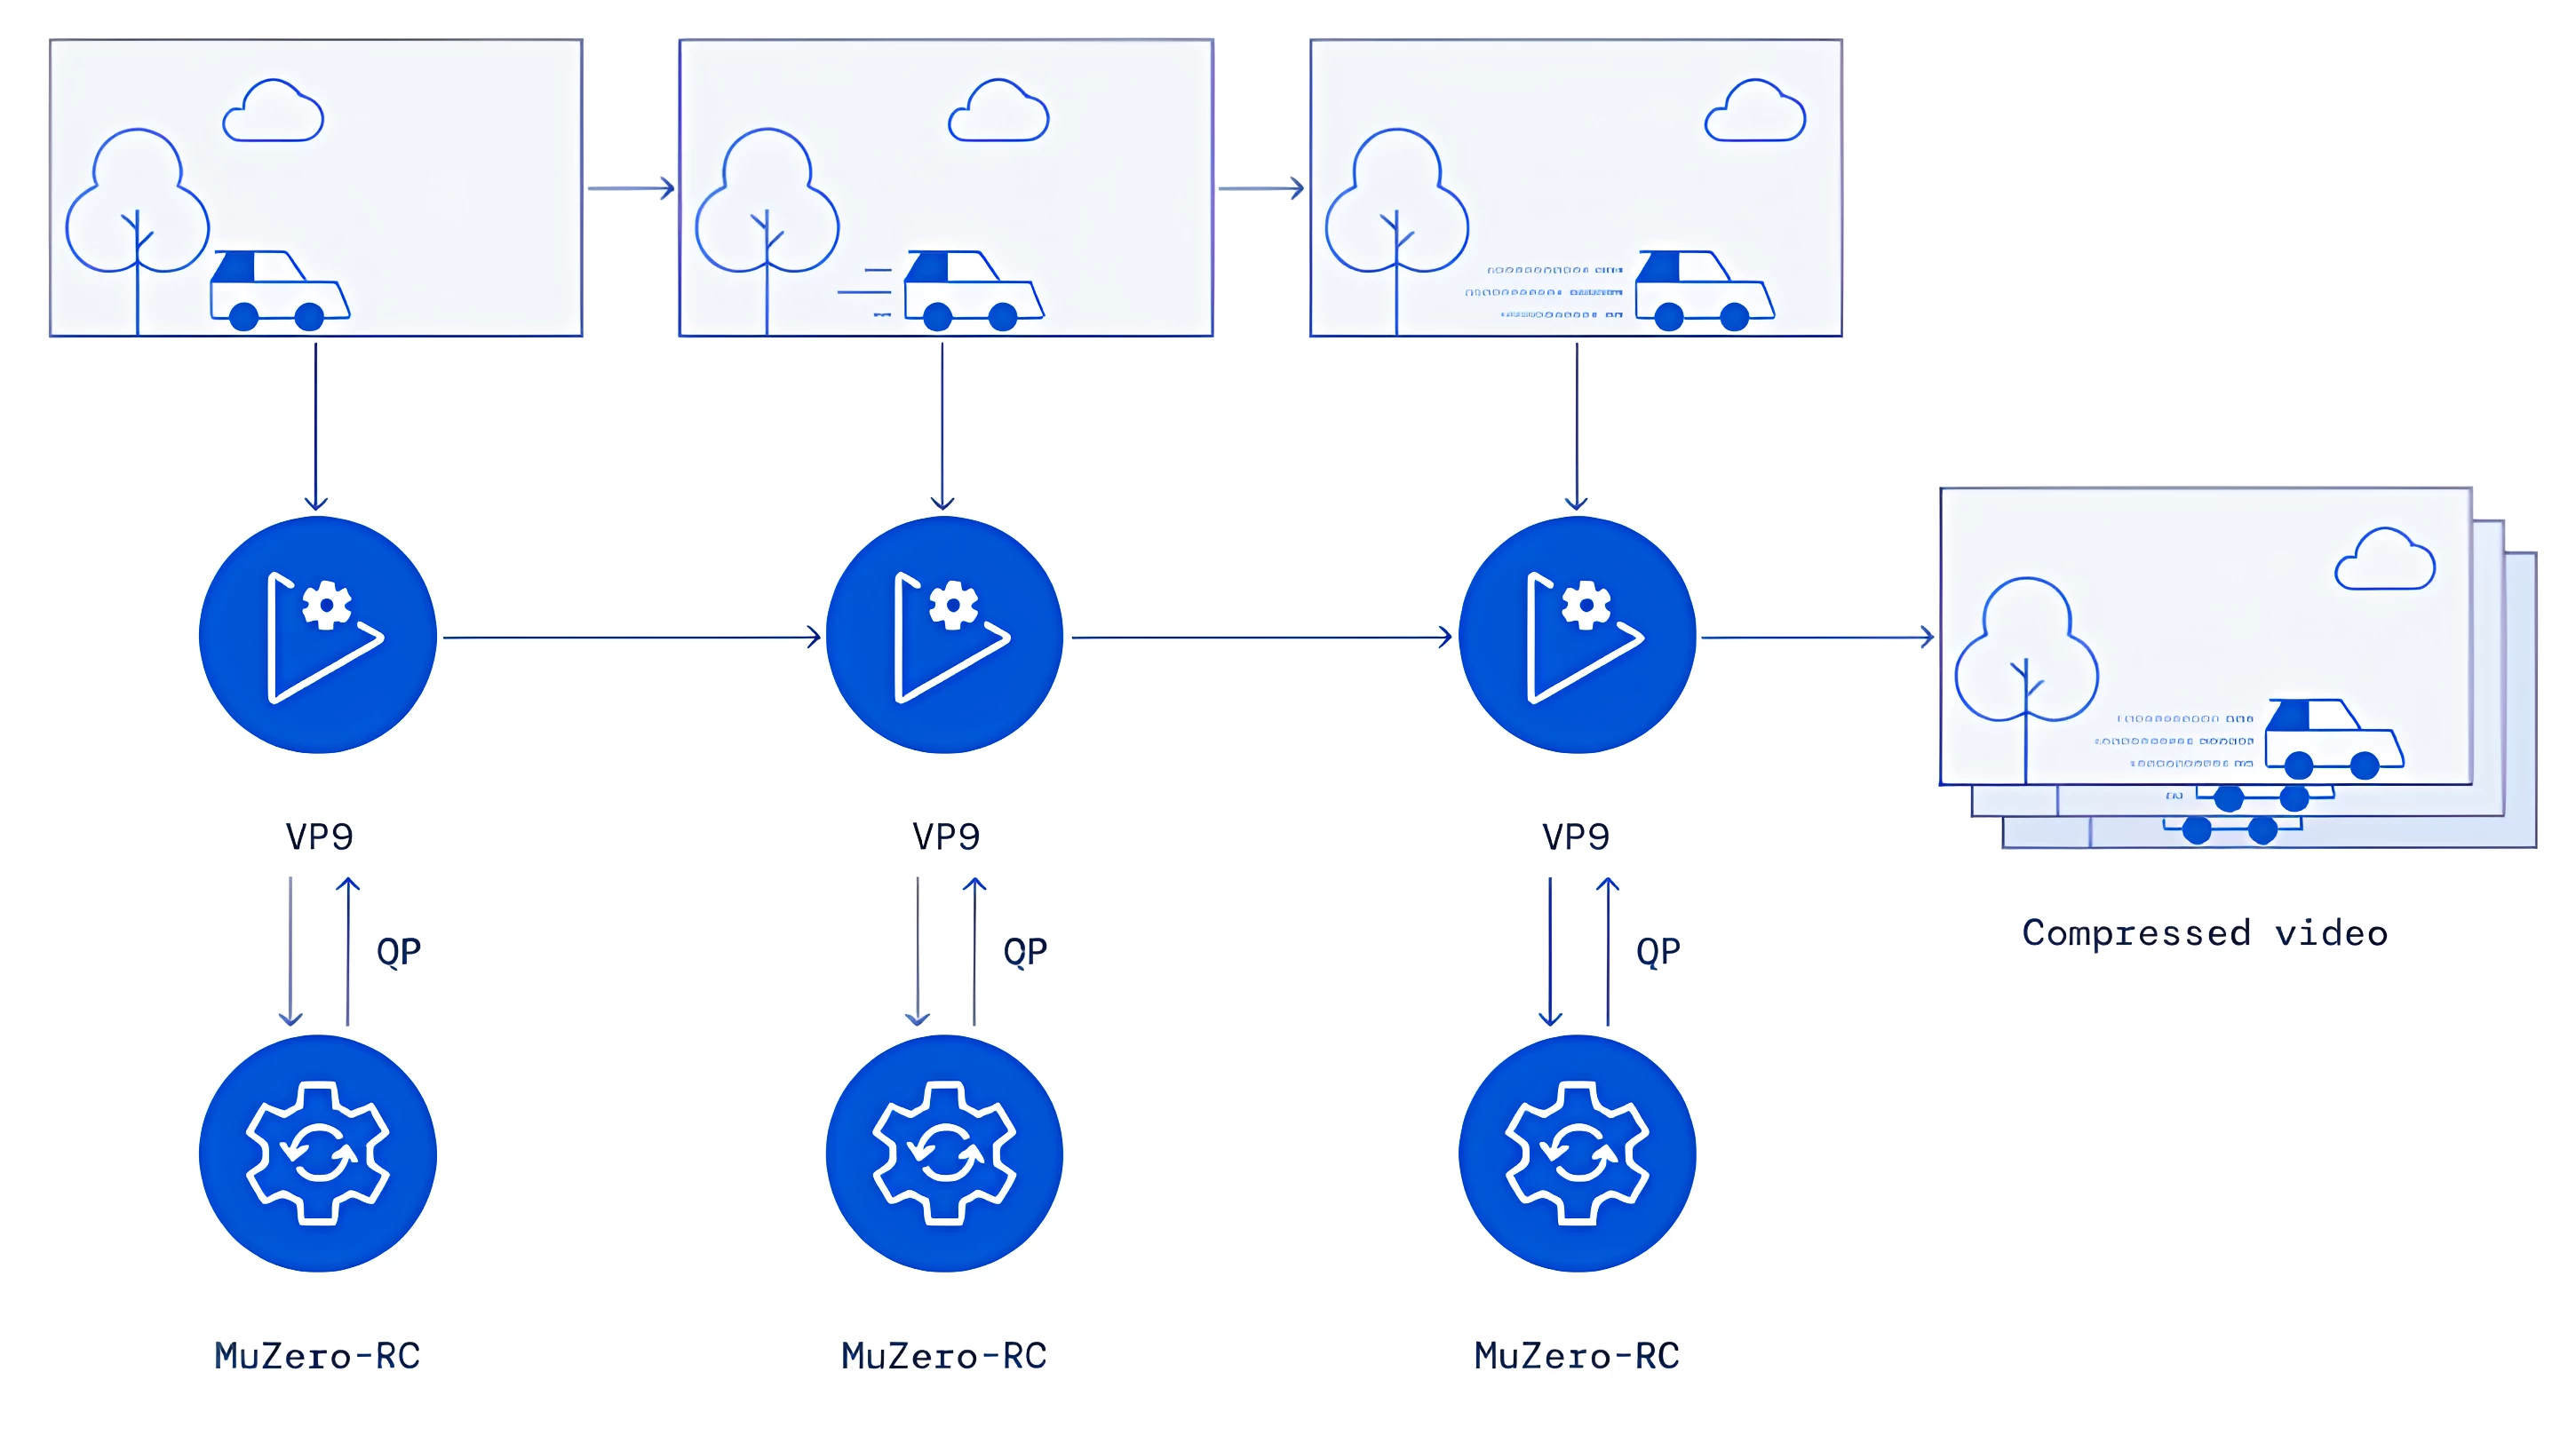
\includegraphics[width=0.7\textwidth]{sections/8Future Directions/MuZeroRC.png}
    \caption{MuZero Rate-Controller (MuZero-RC) optimizing the encoding process in video streaming.}
\end{figure*}

\section{Challenges and Future Directions}
%Future Directions%
As mentioned earlier in the paper, The development of the AI models and
systems in the field of gaming represent a good training set for the 
models to study the environment, address the challenges, modify the 
models, and achieve good results in this field, to judge whether this 
model is able to be implemented in real world, and how it can be implemented. The main purpose 
from such models, Google DeepMind, through the previous years, had been
training the models to play games, and the main goal was to implement the 
models of reinforcement learning in real life, and benefit from them. 
DeepMind already started in this implementation with
MuZero, and developing other models to be able to be implemented in real life 
directly.
\subsection*{MuZero’s first step from research into the real world}
One of the notable implementations of MuZero has been in collaboration 
with YouTube, where it was used to optimize video compression within 
the open-source VP9 codec. This involved adapting MuZero's ability to 
predict and plan, which it had previously demonstrated in games, to a 
complex and practical task of video streaming. By optimizing the 
encoding process, as shown in fig. 3, MuZero achieved an average bitrate reduction of 
4\% without degrading video quality\cite{FD1}. This improvement directly 
impacts the efficiency of video streaming services such as YouTube, 
Twitch, and Google Meet, leading to faster loading times and reduced 
data usage for users. This implementation is called MuZero Rate-Controller (MuZero-RC).
Beyond video compression, this initial application of MuZero outside 
of game research settings exemplifies how reinforcement learning agents 
can address practical real-world challenges. By designing agents with 
new capabilities to enhance products across different sectors, 
computer systems can be more efficient, less resource-intensive, and 
increasingly automated\cite{FD1}.
\begin{figure}[h]
    \centering
    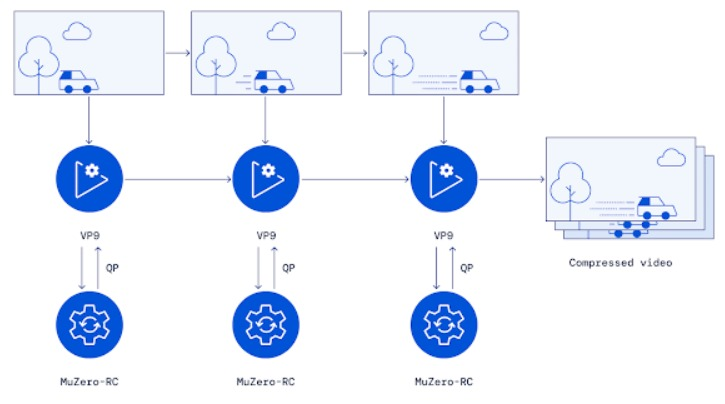
\includegraphics[width=0.4\textwidth]{sections/8Future Directions/MuZeroRC.jpg}
    
    \caption{MuZero Rate-Controller (MuZero-RC) optimizating the encoding process in video streaming.}
\end{figure}
\subsection*{AlphaCode}
AlphaCode is an AI system designed for competitive programming that 
has achieved impressive results. AlphaCode simply leverages 
transformer-based language models to generate code, filtering through 
numerous candidate solutions to identify 
the optimal ones. Its training comes on the basis of
reinforcement learning, which enhances its ability to refine code 
generation strategies. In this framework, AlphaCode generates 
multiple potential solutions for a given problem and evaluates their 
performance against predefined test cases. By rewarding successful 
outcomes and adjusting its approach based on these evaluations, the 
model iteratively improves the quality of its code and explores 
diverse coding strategies. This combination of modeling 
techniques and reinforcement learning not only showcases AlphaCode's 
capability to solve complex problems requiring critical thinking was
able to compete with human programmers, ranking within the top 54\% 
of participants in real-world competitive programming contests\cite{FD2}.
\subsection*{AlphaFold}
AlphaFold is a model developed by DeepMind 
that addresses one of the challenging problems in biology, which is
predicting the three-dimensional structures of proteins from their 
amino acid sequences. AlphaFold employs 
advanced deep learning techniques, prominently featuring 
reinforcement learning, to enhance its predictive capabilities.The 
model operates on a feedback loop where 
it generates predictions about protein structures and receives 
rewards based on the accuracy of these predictions compared to 
experimentally determined structures. This process allows AlphaFold 
to iteratively refine its models, optimizing them to better reflect 
the complexities of protein folding dynamics. The architecture of 
AlphaFold includes deep neural networks that analyze both the 
sequential and spatial relationships between amino acids, enabling 
it to capture intricate patterns for protein conformation. 
By training on extensive datasets of known protein structures, 
AlphaFold has achieved unprecedented accuracy, often rivaling 
experimental methods such as X-ray crystallography and cryo-electron 
microscopy\cite{FD3}.\\\\
As shown form the previous models, how the employment of reinforcementl
learning changed starting from making AI systems which play atari and strategy-based games, 
reaching to help in human biology and create protein structures, the 
enployment of reinforcement learning in games still has a long journey
to be developed which helps in both real life and gaming. Google DeepMind
is still working on other models which are able to be implemented 
in real life applications. They also developed models which use the multi-agent
models in games, like AlphaStar, which is a model to play 
StarCraft II; but still didn't apply them in real life applications, which
is a good future direction to be developed.

\section{Conclusion}
\section*{Conclusion}

Games, as an environment for reinforcement learning, have proven to be very impactful as sandboxes. Their modular nature enables experimentation across different scenarios, ranging from deterministic board games to visually complex and endless Atari games. 

Google’s DeepMind utilized this modularity by developing and enhancing their models incrementally. The progression started with \textbf{AlphaGo}, which relied on human gameplay and explicit knowledge of game rules. This was followed by \textbf{AlphaGo Zero}, which removed the need for human gameplay data, and \textbf{AlphaZero}, which generalized the approach to multiple board games. Finally, \textbf{MuZero} eliminated the requirement for prior knowledge of game rules entirely, achieving breakthrough results in tens of games and surpassing its predecessors.

These advancements have translated into real-world applications, such as \textbf{MuZero’s optimization of YouTube's compression algorithm}, which was already highly optimized using traditional techniques. Similarly, \textbf{AlphaFold}, while inspired by reinforcement learning principles like those in AlphaZero, relies primarily on supervised learning to model complex proteins. 

While these achievements are impressive, especially given their roots in models trained to play simple games, they remain limited in scope. Challenges such as high training costs, scalability, and performance in stochastic environments persist. 

Firstly, these models are \textbf{expensive to train}, even in environments with limited action and state spaces, and this cost only increases in more complex scenarios. Secondly, \textbf{scalability} is another challenge, as many real-world applications involve actions that are not mutually exclusive. This makes techniques like Monte Carlo Tree Search (MCTS) exponentially more expensive. Lastly, these models, while performing well in deterministic settings, may face difficulties when applied to \textbf{stochastic environments}, affecting both training and inference. 

However, ongoing research in areas such as \textbf{model-based reinforcement learning} and \textbf{hierarchical reinforcement learning} provides hope for addressing these limitations, potentially expanding the applicability of these methods to more complex real-world scenarios.



\section*{Acknowledgment}

\section*{References}

Please number citations consecutively within brackets \cite{firstbib}. The
sentence punctuation follows the bracket \cite{b2}. Refer simply to the
reference number, as in \cite{b3}---do not use ``Ref. \cite{b3}'' or
``reference \cite{b3}'' except at the beginning of a sentence: ``Reference
\cite{b3} was the first $\ldots$''

Number footnotes separately in superscripts. Place the actual footnote at the
bottom of the column in which it was cited. Do not put footnotes in the
abstract or reference list. Use letters for table footnotes.

Unless there are six authors or more give all authors' names; do not use ``et
al.''. Papers that have not been published, even if they have been submitted
for publication, should be cited as ``unpublished'' \cite{b4}. Papers that have
been accepted for publication should be cited as ``in press'' \cite{b5}.
Capitalize only the first word in a paper title, except for proper nouns and
element symbols.

For papers published in translation journals, please give the English citation
first, followed by the original foreign-language citation \cite{b6}.

\begin{thebibliography}{00}
    
    
    
    \bibitem{I1}  N. Y. Georgios and T. Julian, Artificial Intelligence and Games. New York: Springer, 2018.
    \bibitem{I2}  N. Justesen, P. Bontrager, J. Togelius, S. Risi, (2019). Deep learning for video game playing. arXiv.
    \bibitem{I3}  V. Mnih, K. Kavukcuoglu, D. Silver, A. Graves, I. Antonoglou, D. Wierstra, M. Riedmiller, (2013). Playing Atari with deep reinforcement learning. arXiv.
    \bibitem{I4}  A. Graves, G. Wayne, I. Danihelka, (2014). Neural Turing Machines. arXiv.
    \bibitem{I5}  C.J.C.H.Watkins, P. Dayan, Q-learning. Mach Learn 8, 279–292 (1992).
    \bibitem{I6}  DeepMind, (2015, February 12), Deep reinforcement learning.
    \bibitem{I7}  T. Schaul, J. Quan, I. Antonoglou, D. Silver, (2015). Prioritized Experience Replay. arXiv.
    \bibitem{I8}  V. Mnih, A. P. Badia, M. Mirza, A. Graves, T. Lillicrap, T. Harley, D. Silver, K. Kavukcuoglu, (2016). Asynchronous Methods for Deep Reinforcement Learning. arXiv.
    \bibitem{I9}  A. Kailash, P. D. Marc, B. Miles, and A. B. Anil, (2017). Deep Reinforcement Learning: A Brief Survey. IEEE Signal Processing Magazine, vol. 34, pp. 26–38, 2017. arXiv.
    \bibitem{I10} D. Zhao,  K. Shao, Y. Zhu, D. Li, Y. Chen, H. Wang, D. Liu, T. Zhou, and C. Wang, “Review of deep reinforcement learning and discussions on the development of computer Go,” Control Theory and Applications, vol. 33, no. 6, pp. 701–717, 2016 arXiv.
    \bibitem{I11} Z. Tang, K. Shao, D. Zhao, and Y. Zhu, “Recent progress of deep reinforcement learning: from AlphaGo to AlphaGo Zero,” Control Theory and Applications, vol. 34, no. 12, pp. 1529–1546, 2017.
    \bibitem{I12} K. Shao, Z. Tang, Y. Zhu, N. Li, D. Zhao, (2019). A survey of deep reinforcement learning in video games. arXiv.
    
    %-------Background-------
    \bibitem{bg1} L. Thorndike and D. Bruce, Animal Intelligence. Routledge, 2017.
    \bibitem{bg2} R. S. Sutton and A. Barto, Reinforcement learning : an introduction. Cambridge, Ma ; London: The Mit Press, 2018.
    \bibitem{bg3} A. Kumar Shakya, G. Pillai, and S. Chakrabarty, “Reinforcement Learning Algorithms: A brief survey,” Expert Systems with Applications, vol. 231, p. 120495, May 2023
    \bibitem{bg4} Mnih, Volodymyr, et al. “Human-Level Control through Deep Reinforcement Learning.” Nature, vol. 518, no. 7540, Feb. 2015, pp. 529–533.
    \bibitem{AD1} T.-R. Wu, H. Guei, P.-C. Peng, P.-W. Huang, T. H. Wei, C.-C. Shih, Y.-J. Tsai, (2023). MiniZero: Comparative analysis of AlphaZero and MuZero on Go, Othello, and Atari games. arXiv.
    \bibitem{AD2} K. Zhang, Z. Yang, T. Ba\c{s}ar, (2021). Multi-agent reinforcement learning: A selective overview of theories and algorithms. arXiv preprint arXiv:2103.04994

\end{thebibliography}
\vspace{12pt}

\end{document}